\documentclass[12pt]{article}
\usepackage{amsmath}
\usepackage{amsfonts}
\usepackage{amssymb}
\usepackage{subfig}
\usepackage{graphicx}
\usepackage{float}

\textwidth 6.5in
\oddsidemargin 0in
\evensidemargin 0in
\textheight 8.6in
\topmargin -0.5in
\pagestyle{empty}
\begin{document}

\vspace*{-1cm}
\begin{center}
{\LARGE \bf Relativistic Quantum Field Theory}

\vspace*{0.5cm}
{\Large Physics 7651} \\
\vspace*{0.5cm}
{\Large {\bf Homework 5}\\
\vspace*{0.5cm}
Due: In class on Wednesday, October 5}
\end{center}
\begin{enumerate}


\item  {\bf Combinatoric factor for external field $S$-matrix} [2 points]

Explain the origin of the combinatoric factor when applying Wick's theorem to an interaction with an external source. 

\item {\bf Unitarity of the $S$-matrix for an external field} [3 points]

Show that the $S$-matrix calculated in class is unitary, that is 
\[ 1 = \sum_n |\langle n|S|0\rangle |^2, \]
where the $\left\{|n\rangle\right\} $ is the set of all possible $n$-particle intermediate states.

\item{\bf Quadratic external field} [15 points]

Consider an interaction Hamiltonian in the presence of an external c-number source as in class, except now assume that the perturbation is quadratic in the field,
$$ H'= \frac{1}{2} \lambda \left[ \int d^3x \rho (\vec{x}) \phi (\vec{x},t)\right]^2,$$
where $\lambda$ is a positive coupling constant and $\rho (\vec{x})$ is a real function of spatial position. Compute the matrix elements $\langle \vec{k}'|S-1|\vec{k}\rangle$ for the scattering between (non-relativistically normalized) one-particle states by summing  connected Wick diagrams. Explicitly verify that the one-particle to one-particle $S$-matrix is unitary. 

%Hints: (1) As discussed in class, you don't need to worry about the disconnected diagrams. (2) Every vertex in a Wick diagram represents a seven dimensional integral: two three-dimensional spatial integrals and one time integral. (3) Don't get carried away by trying to prove mathematical niceties: assume power series converge, $\rho$ is sufficiently smooth and falls of sufficiently rapidly, etc. (4) The final answer involves a single three dimensional integral over momenta involving $\tilde{\rho}(\vec{k})$. Don't try to further simplify it. However if your answer involves more complicated objects you should try to get it to this form.
\textit{Hints:}
\begin{enumerate}
\item[(1)] As discussed in class, you don't need to worry about the disconnected diagrams.
\item[(2)] Every vertex in a Wick diagram represents a seven dimensional integral: two three-dimensional spatial integrals and one time integral.
\item[(3)] Don't get carried away by trying to prove mathematical niceties: assume power series converge, $\rho$ is sufficiently smooth and falls of sufficiently rapidly, etc.
\item[(4)] The final answer involves a single three dimensional integral over momenta involving $\tilde{\rho}(\vec{k})$. Don't try to further simplify it. However if your answer involves more complicated objects you should try to get it to this form.
\end{enumerate}


\vspace*{0.5cm}



\item  {\bf Symmetry factors done honestly} [9 points]

Calculate the symmetry factors for the following \textit{Wick} diagrams `honestly,' that is, expand to the appropriate power of the interaction Hamiltonian and explicitly state all combinatorial factors:
%
\begin{figure}[H]
  \centering
  \subfloat[]{\quad
  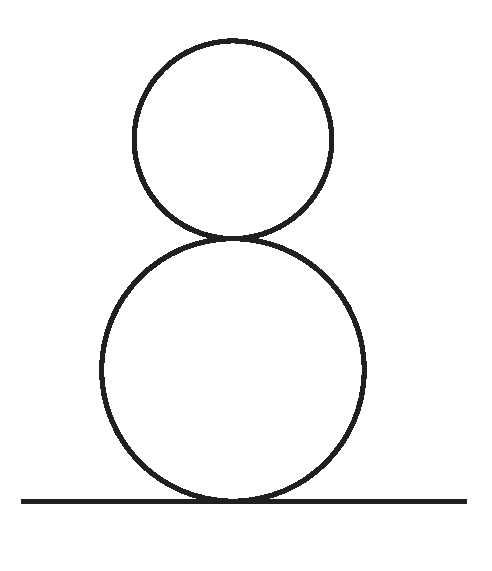
\includegraphics[width=3cm]{hw5_img1}
  \qquad}
  \subfloat[]{\quad
  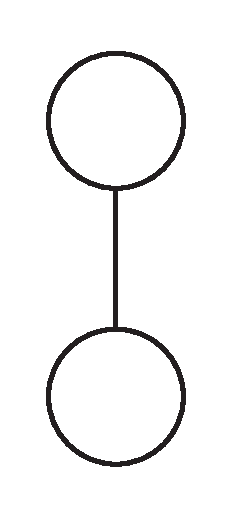
\includegraphics[width=2cm]{hw5_img2}
  \qquad} 
  \subfloat[]{\quad
  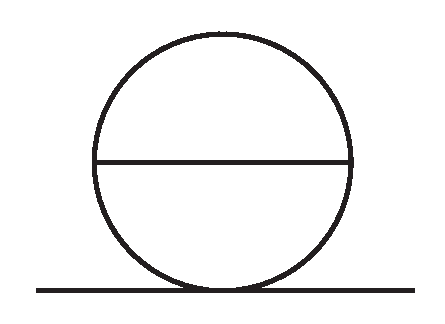
\includegraphics[width=3.3cm]{hw5_img3}
  \qquad}
  \subfloat[]{\quad
  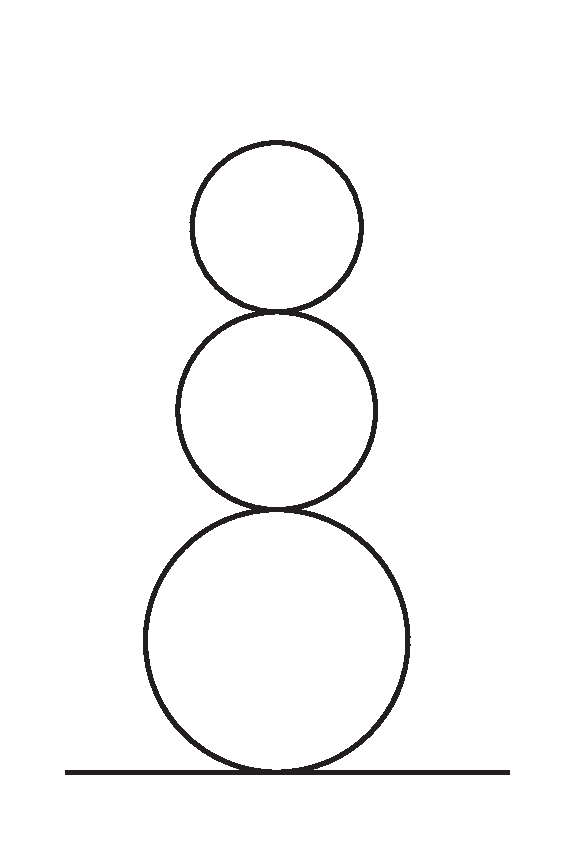
\includegraphics[width=3cm]{hw5_img4}
  \qquad}
\end{figure}
%
Assume the interaction terms take the form $\mathcal L_I = \frac{\lambda_3}{3!} \phi^3 + \frac{\lambda_4}{4!} \phi^4$.
Convince yourself that you get the same results if you work out the symmetry factors the `slick' way. \textit{Hint}: follow the method presented in class since many textbooks define symmetry factors differently (e.g.\ for Wick versus Feynman diagrams). 


\vspace*{0.5cm}



\item  {\bf American Gothic} [1 point]

Determine the symmetry factor of the following Wick diagram based on Grant Wood's \textit{American Gothic}. Assume that the interaction Lagrangian takes the form $\mathcal{L} =\sum_n \frac{\lambda_n}{n!} \phi^n$.
Black dots (eyes) are purely decorative. \textit{Hint}: go ahead and do this the slick way. It helps to simplify the diagram to one that is topologically equivalent.

\begin{center}
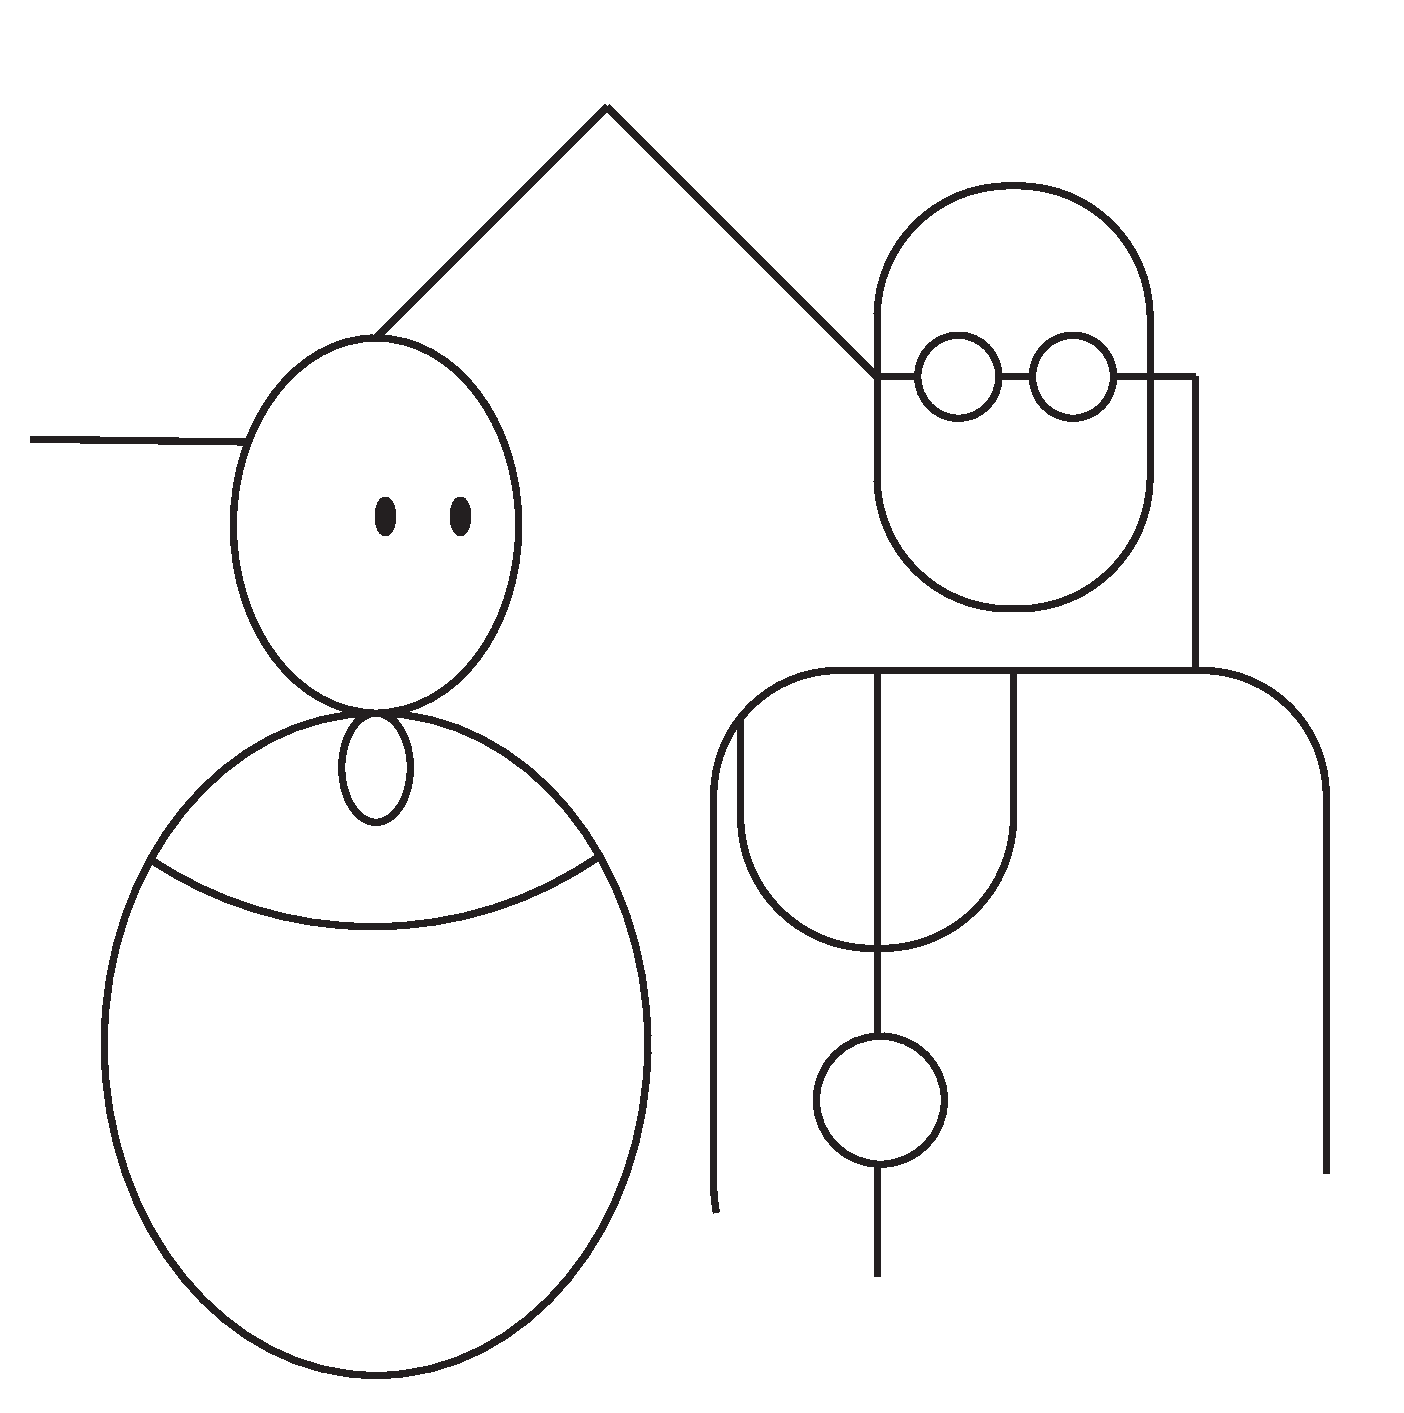
\includegraphics[width=7.5cm]{AmericanGothic}
\end{center}



\end{enumerate}

\end{document}
